\documentclass[../main.tex]{subfiles}
\graphicspath{{\subfix{../images/}}}

\begin{document}


\subsection{Class Distribution}

Both the train and test split have roughly even class 
distributions. Each class making up approximately $20\%$ of the 
data set. 
The training split is slightly less even than the test split, 
with Trouser making up marginally less and T-shirt/top making up 
marginally more, compared to the other classes. Having all 
classes represented somewhat equally benefits us when it comes to 
building our classifiers. We are confident that we have enough 
samples of each class for the model to learn from 
(\autoref{fig:class_dists}). 

\begin{figure}[ht]
    \centering
    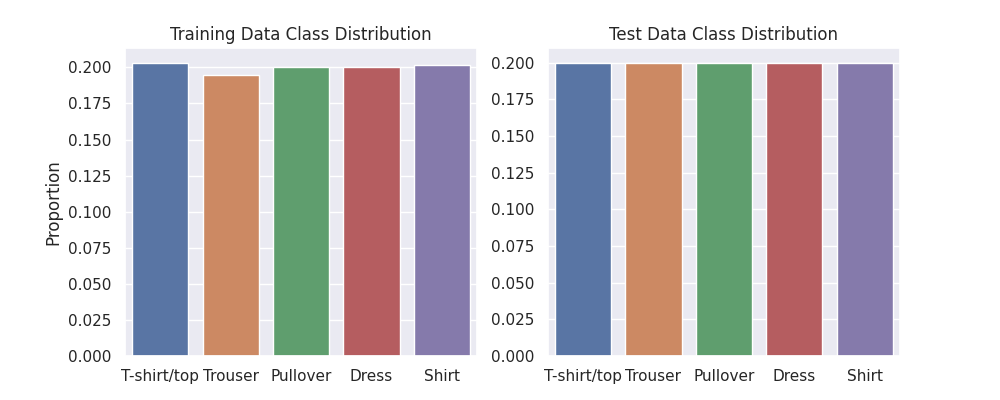
\includegraphics[width=\textwidth]{images/class_distribution .png}
    \caption{Class distribution of train and test split}
    \label{fig:class_dists}
\end{figure}


\subsection{Principle Component Analysis}

Principle Component Analysis (PCA) is an unsupervised machine 
learning method, and is a form of feature extraction which 
compresses the data while maintaining as much of the information 
as possible. We performed PCA and transformed the data further by 
scaling the transformed variables with the square root of the 
eigenvalues. This is a preprocessing step called sphering and it 
transforms the data into a set of new uncorrelated variables with 
variance $1$. With a data set like Fashion MNIST with 784 
features, dimensionality reduction can be very useful for 
transforming the data from a high-dimensional space to a low-
dimensional space.
Dimensionality reduction can improve computational performance, 
improve model performance by avoiding overfitting, and lastly is 
great for visualisation. 

We performed sphering on the unscaled version of the training 
set. We were able to use the unscaled version of the data set, 
since all the features are measured in the same unit. 
From the kernel density function in the pair plot of the first 
five principal components in the train split, it is clear to see 
that there is a lot of class overlap present in the PCA data set 
(\autoref{app:PCA_pairplot}). We would expect that the other 
principal components will portray the same tendency of class 
overlap \autocite{JamesStatisticalLearning}.
This poses a challenge to the classifier, since it becomes 
difficult to distinguish the clothing items from each other.
The first principle component together with the second principle 
component present, what looks like, the clearest class 
separability. 

Looking at the plot of the cumulative explained variance ratio 
(CVR) we see that using only a fraction of the extracted features 
we are still able to preserve a significant amount of the 
information in the original data set, in terms of explained 
variance (\autoref{fig:cvr_pca}). In fact, we are able to 
preserve $90\%$ of the explained variance with the first $62$ 
principal components. This is a reduction of the feature space by 
$92\%$.

\begin{figure}[ht]
    \centering
    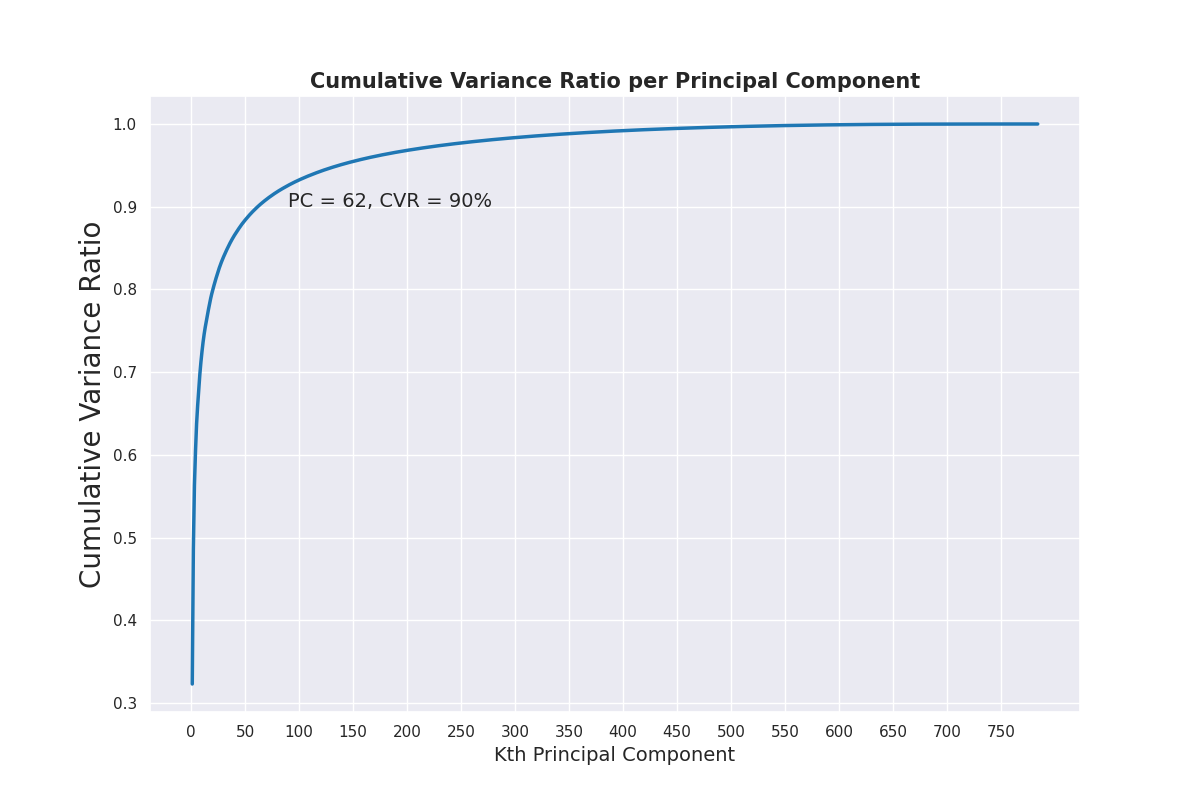
\includegraphics[width=0.7\textwidth]
    {images/CumVarianceRatio_PCA.png}
    \vspace*{-5mm} % til at få catption tættere på plottet
    \caption{Plot of the cumulative variance ratio for the 
    principal components}
    \label{fig:cvr_pca}
\end{figure}


\end{document}